%;whizzy document -pdf -initex "pdflatex -ini" -latex pdflatex
\documentclass[a4paper,10pt]{article}
%\usepackage[T1]{fontenc}
\usepackage{setspace}
\usepackage[vmargin=1in,hmargin=1.25in]{geometry}
\usepackage[T1]{fontenc}
\renewcommand*\familydefault{\sfdefault}
\usepackage{hyperref}
\usepackage{mdwlist}
\usepackage{fullpage}
\usepackage[cmex10]{amsmath}
\usepackage[portuguese]{babel}
\usepackage[utf8]{inputenc}
\usepackage{graphicx}
\hypersetup{
pdftitle={Códigos de linha e de scrambling},
pdfauthor={Renan Birck Pinheiro}
}
\title{Códigos de linha e de \textit{scrambling}}
\author{Renan Birck Pinheiro}
\date{\today}

\begin{document}
\maketitle

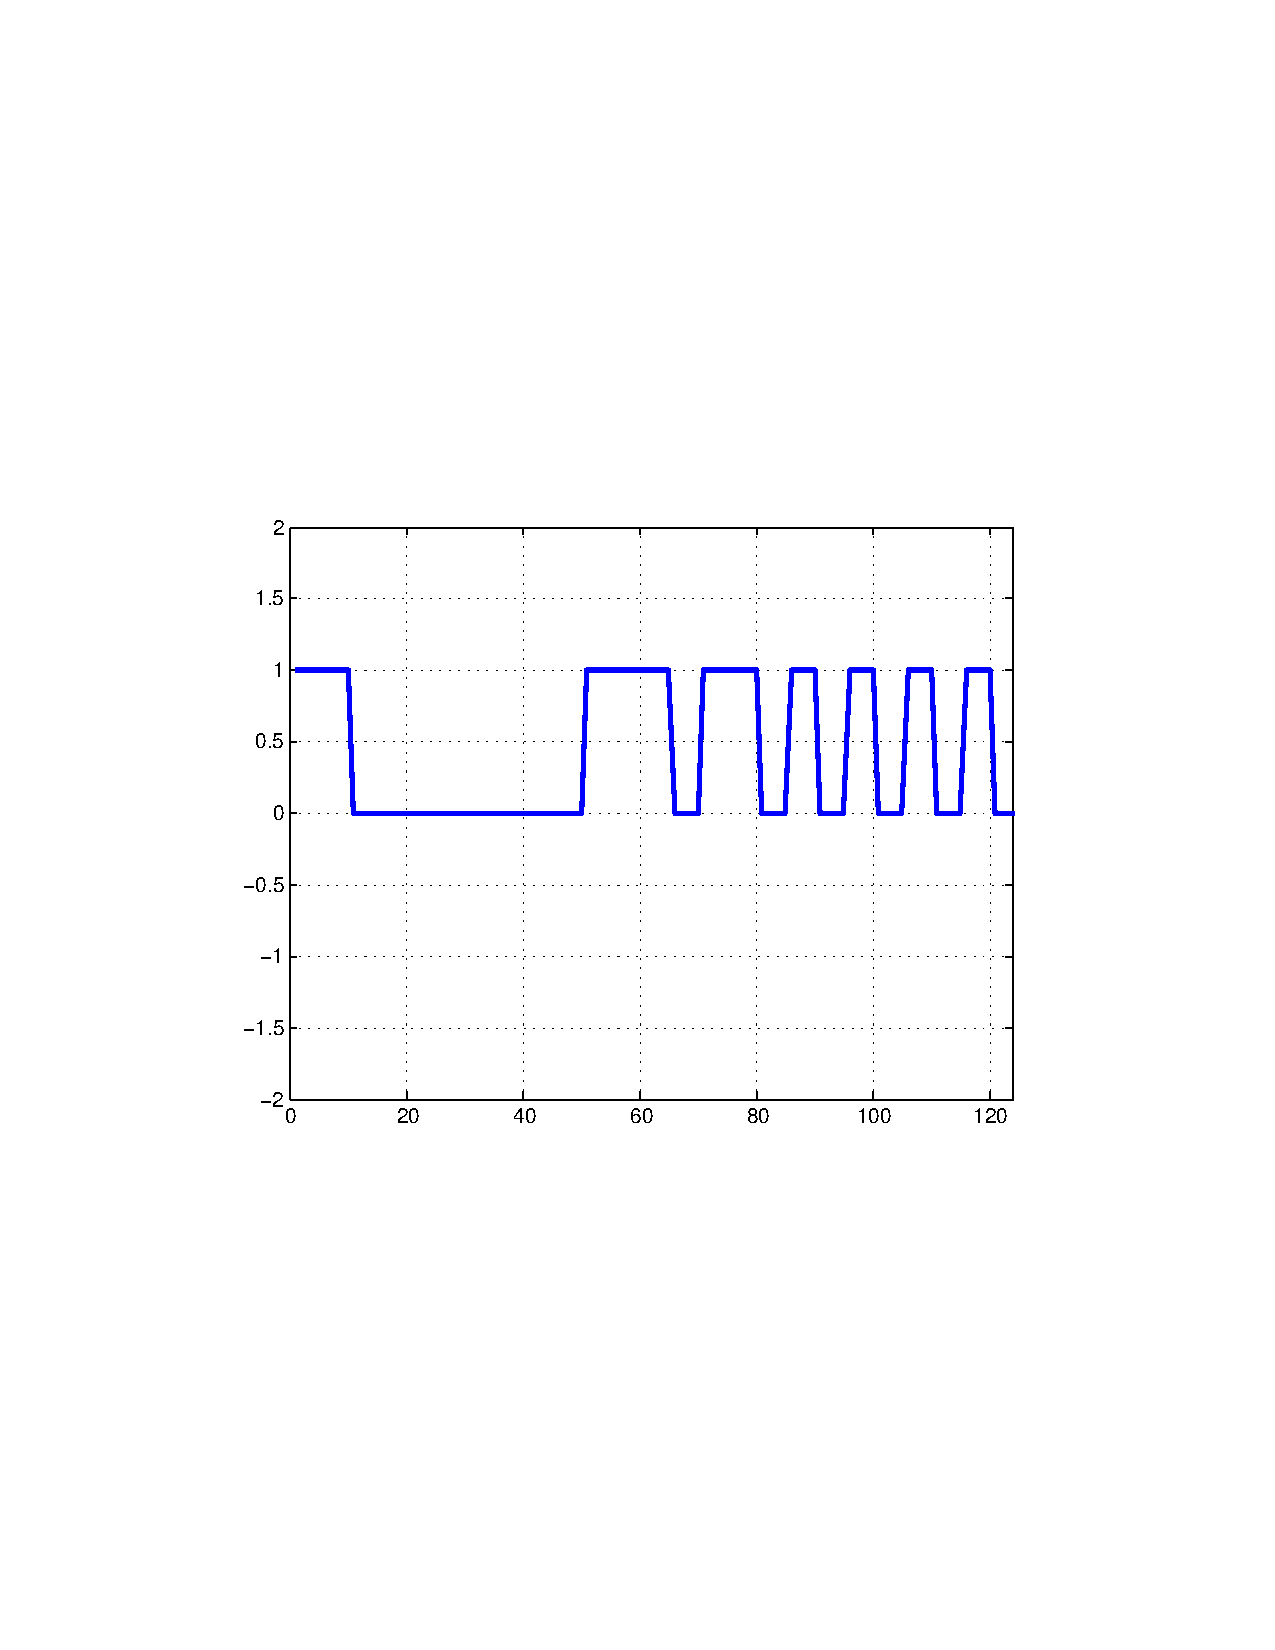
\includegraphics{bitstream.pdf}
\begin{thebibliography}{99}
\bibitem[1]{NotasAula} MACHADO, R. {\bf Notas de aula da disciplina de Transmissão e Comunicação de Dados}. Disponível em \url{http://www.ufsm.br/gpscom/professores/Renato\%20Machado/comunicacaodedados.html}. Acesso em 28/04/2012.
\end{thebibliography}
\end{document}          
